\documentclass[a4paper]{scrreprt}

% Uncomment to optimize for double-sided printing.
% \KOMAoptions{twoside}

% Set binding correction manually, if known.
% \KOMAoptions{BCOR=2cm}

% Localization options
\usepackage[english]{babel}
\usepackage[T1]{fontenc}
\usepackage[utf8]{inputenc}

% Sub figures
\usepackage{subcaption}

% Quotations
\usepackage{dirtytalk}

% Floats
\usepackage{float}

% Enhanced verbatim sections. We're mainly interested in
% \verbatiminput though.
\usepackage{verbatim}

% Automatically remove leading whitespace in lstlisting
\usepackage{lstautogobble}

% CSV to tables
\usepackage{csvsimple}

% PDF-compatible landscape mode.
% Makes PDF viewers show the page rotated by 90°.
\usepackage{pdflscape}

% Advanced tables
\usepackage{array}
\usepackage{tabularx}
\usepackage{longtable}

% Fancy tablerules
\usepackage{booktabs}

% Graphics
\usepackage{graphicx}

% Current time
\usepackage[useregional=numeric]{datetime2}

% Float barriers.
% Automatically add a FloatBarrier to each \section
\usepackage[section]{placeins}

% Custom header and footer
\usepackage{fancyhdr}

\usepackage{geometry}
\usepackage{layout}

% Math tools
\usepackage{mathtools}
% Math symbols
\usepackage{amsmath,amsfonts,amssymb}
\usepackage{amsthm}
% General symbols
\usepackage{stmaryrd}

% Utilities for quotations
\usepackage{csquotes}

% Bibliography
\usepackage[
  style=alphabetic,
  backend=biber, % Default backend, just listed for completness
  sorting=ynt % Sort by year, name, title
]{biblatex}
\addbibresource{references.bib}

\DeclarePairedDelimiter\abs{\lvert}{\rvert}
\DeclarePairedDelimiter\floor{\lfloor}{\rfloor}

% Bullet point
\newcommand{\tabitem}{~~\llap{\textbullet}~~}

\pagestyle{plain}
% \fancyhf{}
% \lhead{}
% \lfoot{}
% \rfoot{}
% 
% Source code & highlighting
\usepackage{listings}

% SI units
\usepackage[binary-units=true]{siunitx}
\DeclareSIUnit\cycles{cycles}

% Should use this command wherever the print date is mentioned.
\newcommand{\printdate}{\today}

\newcommand{\mailsubject}{Privacy and Data Security - Summary}
\newcommand{\maillink}[1]{\href{mailto:#1?subject=\mailsubject}
                               {#1}}

\subject{Privacy and Data Security}
\title{Summary}

\author{Michael Senn \maillink{michael.senn@students.unibe.ch} --- 16-126-880}

\date{\printdate}

% Needs to be the last command in the preamble, for one reason or
% another. 
\usepackage{hyperref}

\begin{document}
\maketitle

\chapter{Computer security}

\begin{itemize}
		\item Quine: Program printing its own source code
		\item Reflections on trusting trust: Compiler inserting backdoors into
				compilers and target program.
		\item Real-world security usually with layers
\end{itemize}

\section{Access control}

\begin{description}
		\item[Subject] Requests access to resource
		\item[Resource] Entity being accessed by subject
		\item[Policy] Specifies how subject may access request
				\begin{description}
						\item[Column-based] Each resource specifies what
								subjects allowed to access. Compare ACL, Linux
								file system.
						\item[Row-based] Each subject knows which resources it
								is allowed to access. Protection required as
								subjects untrusted. E.g. keycards with
								public-key crypto.
						\item[Full matrix] Mapping of subject to resource. E.g.
								sudoers file.
				\end{description}
		\item[Reference monitor] Evaluates whether request by subject to
				resource is conformant with policy
\end{description}

\chapter{Tracking}

\begin{description}
		\item[Worth of data] Pure data companies: One person's data's worth
				about 10-15 USD per year
		\item[First vs third party cookies] Set by visiting site, vs set by external content loaded by that site
		\item[Evercookie] Collection of various storage mechanics to store
				persistent identifier. Flash, HTML5 local storage, etags, ...
		\item[Server-sided cookie synchronization] Site A sets cookie and loads
				third-party resource rom site B, including site-A-ID in that
				request. Site B can then set cookie and knows relation to site
				A.
		\item[Passive tracking] E.g. browser fingerprinting: Fonts, canvas rendering, devices, ...
\end{description}

\chapter{Anonymization}

\begin{itemize}
		\item Eliminate personal data while keeping utility high
		\item Challenge: Correlation of anonymized with external data
\end{itemize}

\subsection{K-anonymity}

Given data set $A$, partition its attributes into classes:
\begin{itemize}
		\item $S$ sensitive attributes, those an adversary wants to learn (e.g. health status)
		\item $I$ identifiers, which identify individual (e.g. SSN). Removed before dataset published.
		\item $QI$ quasi-identifiers, which can help to identify individual (e.g. birth date)
\end{itemize}

A dataset is $k$-anonymous if each partition of the dataset, grouped by its QI,
has at least $k$ members. $k$ elements must \emph{not} be distinct.

\begin{description}
		\item[Supression] Remove infrequent values of QI fields
		\item[Generalization] Replace QI values with more generic ones. Numerical ranges, categorical hierarchies, ...
\end{description}

Problems:
\begin{description}
		\item[Background knowledge] E.g. knowing non-QI data about target person can allow correlation
		\item[Homogenity attack] If all members of partition have equal sensitive attributes, can still learn them
\end{description}

\subsection{L-diversity}

Equivalence class is l-diverse if it contains at least $l$ well-represented
values of sensitive attributes. Dataset is $l$-diverse if all its equivalence
classes are $l$-diverse.

``Well-represented'':
\begin{description}
		\item[Distinct $l$-diversity] Sensitive attributes take on at least $l$ distinct values
		\item[Probabilistic $l$-diversity] Proportion of each attribute at most $\frac{1}{l}$.
\end{description}

Probabilistic implies distinct, stronger assumption.

Problems:
\begin{description}
		\item[Homogenity] attack still possible
		\item[Skewed data set] If sensitive data has one unlikely attribute
				(e.g. HIV+), and equivalence class has significantly higher
				ratio of it, then an individual being part of equivalence class
				implies information. (A posterior != a priori)
\end{description}

\chapter{Epsilon closeness}

Given a dataset $A$ with sensitive attributes $S = \{s\}$. Let $P_Q$ be
empirical distribution of $S$ in dataset, that is:

\[
		P_Q(s) = \frac{\abs{\{c \in A : S = s\}}}{\abs{C}}
\]

And $P_L$ distribution of $S$ over an equivalence class $L$.

Then $L$ is $\epsilon$-close to the whole dataset if:
\[
		D(P_L, P_Q) \leq \epsilon
\]

For a distance function $D$.

The whole dataset is $\epsilon$-close if all of its equivalence classes are
$\epsilon$-close.

\subsection{$n-\epsilon$-close}

An equivalence class is $n-\epsilon$-close to the full dataset if there exists
a subset $M$ of the dataset, with $\abs{M} \geq n$, and $D(P_L, P_{Q | M}) \leq
\epsilon$.

A partition $C$ is $n-\epsilon$-close to th full dataset if there exists a
subset $M$, $\abs{M} \geq n$, such that \emph{each} equivalence class $L$
satisfies the above.

\chapter{Differential privacy}

Given $n$ values $x_1, x_2, \ldots, x_n$ corresponding to secret values of $n$
individuals, where $X = \{0, 1\}$ or $X \subset \mathbb{N}$.

A randomized algorithm $M : X^n \rightarrow Y$ sanitizes a vector $x^n \in X^n$
and outputs $y \in Y$.

Two datasets $x^n, x'^n$ are \textbf{neighbouring} if they differ in exactly
one element. Notation: $x^n \sim x'^n$.

$M$ has $\epsilon$-\textbf{differential privacy} if, for all $Y' \subset Y$, for all $x^n \sim x'^n$:
\[
		P(M(x^n) \in Y') \leq e^\epsilon \cdot P(M(x'^n) \in Y')
\]

\begin{itemize}
		\item Algorithm $M$ necessarily randomized to achieve DP.
		\item $\epsilon$ is privacy parameter. The smaller, the more private.
				Usually in $[0.1, 0.5]$.
		\item One entry in dataset affects output by at most $e^\epsilon$
		\item In practice: Might have trusted party running $M$. Or MPC.
		\item DP is additive. $e^{\epsilon_1} \cdot e^{\epsilon_2} = e^{\epsilon_1 + \epsilon_2}$
		\item Anonymization locally: ``Local differential privacy''. No need
				for trusted party, but requires clients to be honest, and
				anonymized dataset has less utility.
		\item Anonymization by trusted party: Higher utility of anonymized
				dataset, need not trust clients, but requires trusting
				anonymizing party.
\end{itemize}

% TODO study randomized response algorithm, and proof that it is epsilon-DP

\section{Laplace mechanism}

Goal: Apply noise from laplace distribution to achieve DP.

Let $f : X^n \rightarrow Y$ be query function on dataset. $N \in Y$ random
noise. Define $M(X^n) = f(X^k) + N$. Noise $N$ should have mean $0$ to not
affect mean of data.

Let $\Delta = \abs{f(X^n) - f(X'^n)}$. For DP it is required that:
\[
		P(N = y) / P(N = y + \Delta) \leq e^\epsilon
\]

That is, $\Delta$ ensures that, if output of query function changed by at most
$\Delta$, then probability ratio changes by at most $e^\epsilon$.

\subsection{L1 sensitivy}

L1 sensitivy of query function $f : X^n \Rightarrow \mathbb{R}^k$ is:
\[
		\Delta^{(f)} = \max_{X, X' \text{ neighbouring}} \{||f(X^n) - f(X'^n)||_1\}
\]

\begin{itemize}
		\item L1 sensitivity of $f(X^n) = mean(X^n)$: $\Delta^{(f)} = 1/n$
\end{itemize}

\subsection{Laplace distribution}

Random value $X \sim \operatorname{Lap}(b)$ is a Laplace distribution with PDF:
\[
		P(X = x) = \frac{1}{2b} \cdot e^{-\frac{\abs{x}}{b}}
\]

And variance:
\[
		\operatorname{Var}(X) = 2b^2
\]

\subsection{Laplace mechanism}

Given query function $f : X^n \Rightarrow \mathbb{R}^k$, Laplace mechanism $M :
X^n \Rightarrow \mathbb{R}^k$ is:
\begin{align*}
		M(X^n) = f(X^n) + \{N_1, N_2, \ldots, N_k\} \\
		N_i \sim \operatorname{Lap}(\frac{\Delta}{\epsilon}), \text{ IID}
\end{align*}

\subsubsection{Example: Mean}

Let $f(X^n) = \operatorname{mean}(X^n)$. Thus:

\begin{align*}
		Y = M(X^n) & = f(X^n) + \operatorname{Lap}(\frac{\Delta}{\epsilon}) \\
				   & = f(X^n) + \operatorname{Lap}(\frac{1}{\epsilon n})
\end{align*}

\subsubsection{Example: Counting}

Let $f$ be counting query, that is $f(X^n)$ is number of $x \in X^n$ such that
a certain predicate holds. Clearly $\Delta^{(f)} = 1$, as changing any value of
a vector $x \in X^n$ will change the result of the counting query by at most 1.

\subsubsection{Example: Histogram}

Let $f$ be histogram. Then, $\Delta^{(f)} = 2$, as at most one item moves from
one bucket to another.

\chapter{Machine learning for privacy, Privacy for machine learning}

Privacy criteria:
\begin{description}
		\item[Singling out] Isolating some or all records of an individual
		\item[Linkability] Linking multiple records of one individual or group
		\item[Inference] Deducing value of one attribute from values of other
				attributes
\end{description}

Privacy attacks:
\begin{description}
		\item[Linkability/Reidentificatin] Achieve linkability or singling out (`X and Y are both records of Z')
		\item[Attribute inference] Achieve inference of attributes (`X's age is Y')
		\item[Membership inference] Achieve inference of dataset membership (`Is X in Dataset Y')
\end{description}

\section{Example attacks in genomics}

\subsection{Attribute inference}

\begin{itemize}
		\item OpenSNP: Individuals can share their genetic information
		\item Social networks allow finding relatives of target person
		\item Build a priori model based on observations of public
		\item Known inter- and intra-genome correlation due to family ties
		\item Belief propagation in Bayesian networks
\end{itemize}

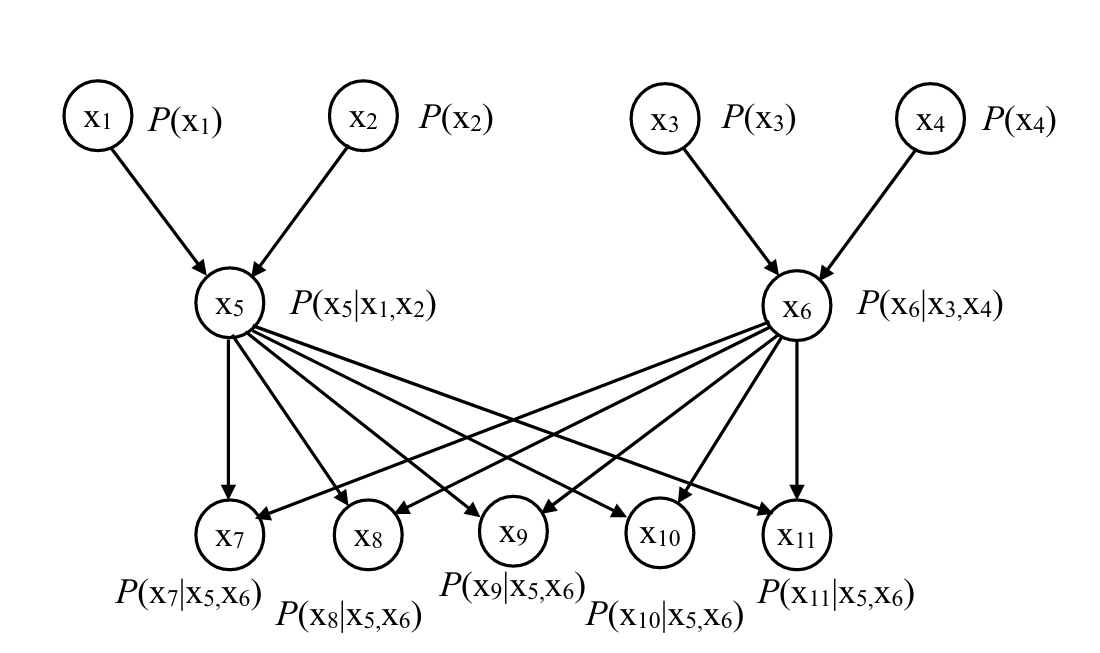
\includegraphics[width=0.6\textwidth]{resources/8_bayesian_network}

\begin{itemize}
		\item Similar model/attack feasible with e.g. physical location. Social
				networks often include location inormation.
		\item Traditional approach would be hidden Markov model but does not
				scale well with highly correlated systems. Bayesian network
				better suited.
\end{itemize}

\subsection{Linkability / re-identification}

\begin{itemize}
		\item Genome: Fixed over time. miRNA expression: Highly variable
		\item Goal: Based on two datasets with miRNA expression, identify records of same individual
		\item Datasets based on either expression in plasma, or blood
		\item Up to 90 percent (for blood-based miRNA samples) could be linked across datasets
		\item Increasing size of dataset causes sharp (plasma) or linear (blood) decrease in linkability
		\item Defense mechanisms: Hiding non-relevant miRNA expression or randomizing shown ones
		\item Hiding low number of miRNAs allowed to reduce linkability attacks
				by half, while only affecting diagnostics by one percent
\end{itemize}

\chapter{Differential privacy (cont)}

\section{Properties of DP}

Seen before: Postprocessing preserves DP. Now: Sequential composition.

\subsection{Sequential composition}

Let $M_1 : X^n \rightarrow Y$, $M_2 : X^n \times Y \rightarrow Z$. If $M_1$ is
$\epsilon_1$-DP and $M_2$ is $\epsilon_2$-DP, then $M_1 \circ M_2$ has
$\epsilon_1 + \epsilon_2$-DP.

Proof: Straight-forward, insert composition into definition of DP, use
$\epsilon$-DP of respective operations.

\subsection{Group privacy}

If $X^n$, $X'^n$ differ in $b$ positions, there exists a sequence of $b$
$X_i^n$ differing in one element each. Then, for $M$ with $\epsilon$-DP, $M$
has $b \epsilon$-DP.

\section{DP and private machine learning}

If dataset has $\epsilon$-DP, then no ML algorithm running on it will violate
that. Issue is always the improperly anonyized dataset, which can be abused by
ML algorithm. Example: Netflix dataset of 'anonymized' views or US retailer
learning people are pregnant before they themselves do.

\section{DP in practice}

Practical issues:
\begin{enumerate}
		\item Obtained metrics must be represented as bit strings for reporting
				purposes
		\item Values might not change a lot over time, simple (repeated) DP
				collection would reveal too much as noise could be avgd out
		\item Data must be collected efficiently
\end{enumerate}

\subsection{Bloom filters (solution to 1)}

Bloom filter $B$ is $m$-length bitstring. Define $l$ hash functions $H_1,
\ldots, H_l$ which uniformly map elements $x \in X$ to $[1, m]$. Let $X$ be set
of encoded values one wants to store.

To add $x \in X$ to $B$, calculate $h_i = H_i(x)$ for all $i$, and set those
bits of $B$ which $h_i$ evaluated to.

Set membership then has no false negatives, but can have false positives.

$B$ can then be randomized before sending.

\subsection{Memoization (solution to 2)}

Do not report new $\epsilon$-DP $B'$ on every report. Rather, memoize it and
report same one as long as $B$ did not change.

RAPPOR paper:
\begin{itemize}
		\item Bloom filter $B$
		\item On change, calculate $B'$ using deterministic (based on client and $B$) noise
		\item On report, calculate $B''$ based on $B'$ using randomized noise and report
		\item Deterministic noise ensures that, while randomized noise of $B''$
				can be avgd out, one still only gets $B'$
		\item Randomized noise ensures that different reports never contain
				same $B'$, which would otherwise allow to link those as being
				of the same person
\end{itemize}

\subsection{Efficient data collection (solution to 3)}

\begin{itemize}
		\item Each user reports $x_i \in [0, m]$, for $i = 1, \ldots, n$
		\item Local laplace mechanism: $Y_i = X_i + \operatorname{Lap}(m/e)$
		\item Sending one bit $Y_i$ with certain probability -> BKY17 paper
\end{itemize}

\chapter{Pseudonymization}

\begin{itemize}
		\item Pseudonymization ensures data can no longer be linked to person,
				except with additional information
		\item Compare: Anonymous data can no longer be linked to data subject
				at all
		\item Uses in testing, analytics, legal attack etc
\end{itemize}

Methods:
\begin{description}
		\item[Encrypt of dataset] Fully secure but no utility. E.g. for backups
		\item[Reduction or masking] Loss of utility
		\item[Irreversible tokenization] (Via e.g. one-way function,
				collision-free map.) Preserves structure, may preserve format.
		\item[Reversible tokenization] (Via e.g. symmetric encryption).
				Preserves structure, may preserve format.
\end{description}

\section{Security model}

\begin{description}
		\item[Dataset] Contains table with fields
		\item[Tokenization] Process with key $K$, consumes dataset. Performed
				by trusted party.
		\item[Pseudonymized dataset] Output of tokenization. Accessed by
				untrusted party.
\end{description}

\section{Table lookup}

\begin{itemize}
		\item Random values as tokens
		\item Store all mappings
		\item Reversible, costly
\end{itemize}

\section{Irreversible tokenization}

Unkeyed with hash:
\begin{itemize}
		\item Hash function $H: \{0, 1\}^* \rightarrow \{0, 1\}^k$, collision
				resistance, first and second preimage resistance
		\item Tokenization as $y = H(x)$ for personal information $x$
		\item Vulnerable to a) enumeration attack and b) lookup of specific $x$
\end{itemize}

Keyed with PRF:
\begin{itemize}
		\item PRF $F: \{0, 1\}^\lambda \times \{0, 1\}^m \rightarrow \{0, 1\}^k$
		\item Tokenization as $y = F_k(x)$ for secret key $k$, personal information $x$
		\item Additional security over unkeyed tokenization
\end{itemize}

\subsection{Format-preserving tokenization: Cycle-walking algorithm}

\begin{itemize}
		\item Data often has structure, e.g. CC numbers, IBAN, ...
		\item Crypto primitives output unstructured outupt (or output with
				different structure)
		\item Let structure be denoted by set $M \subset T$, with efficient
				test for $x \in M \forall x \in T$
		\item Assume $|T| = O(|M|)$, that is roughly `equal' size. Otherwise,
				truncate output of $F$.
\end{itemize}

Given cryptographic prmitive $F : T \rightarrow T$, collision-free. Then:

\begin{lstlisting}[mathescape=true]
map(F, s):
  t = s // $s \in M$
  do:
    t = F(t)
  until $t \in M$

  return t

unmap($F^{-1}$, t):
  s = t // $s \in M$
  do:
    s = $F^{-1}(s)$
  until $s \in M$

  return s
\end{lstlisting}

Assuming $F$ is collision-free, then
$\operatorname{unmap}(\operatorname{map}(x)) = x \forall x \in M$.

\section{Reversible tokenization}

Goal: Starting with block cipher with output domain $C$, where $|C| = 2^k$,
encrypt values of domain $T$, where $|T| = N$ for arbitrary $N < 2^k$.

Let $a, b \in \mathbb{N}$ with $ab \geq N$, $T = \{0, 1, \ldots, N - 1\}$.
Given a PRF $B : K \times \{0, 1\}^* \rightarrow \{0, 1\}^k$.

\begin{lstlisting}[mathescape=true]
FE-Enc(z, a, b, m): // $z \in K$ key, $m \in T$ message
  $L_0 = m \operatorname{div} b$
  $R_0 = m \operatorname{mod} b$
  
  for i = 1 .. rounds:
    if i odd:
	  s = a
    else:
	  s = b
    
	$L_i = R_{i-1}$
	$R_i = (L_{i-1} \oplus B(z, i || R_{i-1})) \operatorname{mod} s$

  return $s \cdot L_{rounds} + R_{rounds}$ // $\in {0, 1, \ldots, ab - 1}$
\end{lstlisting}

Decryption accordingly, in reverse.

\subsection{Format-preserving encryption}

Format-preserving encryption then uses the FE-Enc above plus cycle-walking.

\chapter{Steganography}

Goal: Hide existence of communication. Compare:

\begin{description}
		\item[Cryptography] Hides content of information, but presence known
		\item[Steganography] Hides presence of information.
		\item[Watermarking] Embed information in robust way. Presence known,
				but difficult to remove.
		\item[Fingerprinting] Like watermarking, but user-specific.
\end{description}

\section{Formal model}

\begin{description}
		\item[Alice, Bob] communicating parties
		\item[Secret key $sk$] Communicated out-of-band between Alice and Bob
		\item[Adversary] Able to listen to all messages exchanged between the
				parties. Passive only.
		\item[Covertext $C$] Allowed communication, over domain $Y$
		\item[Stegotext $S$] Communication with embedded message, over domain $Y$
\end{description}

Adversary aims to distinguish stegotext $S$ from covertext $C$. Adversary knows
distribution of covertexts, $C$ modelled as random variable.

\section{Information-theoretic security}

Adversary distinguishes stegotext from covertext with distinguisher $D$.
Qualified using relative entropy:
\[
		D(P_C | P_S) \leq \epsilon
\]

For $\epsilon = 0$ perfect security. Else, statistical security.

Relative entropy:
\[
		D(P_C | P_S) = \sum_{y \in Y} P(C = y) \cdot \log_2(P(C = y) / P(S = y)) \geq 0
\]

\subsection{Bounds on detection}

Deciding $S$ with input $C$ is type-1 error (false positive), probability
$\alpha$. Deciding $C$ with input $S$ is type-2 error (false negative),
probability $\beta$.

Statistical security:
\[
		D(P_C | P_S) \leq \epsilon
\]

For $\alpha = 0$ this implies:
\[
		\beta \geq 2^{-\epsilon}
\]

In words: If we want no false positives, we cannot get the probability of false
negatives arbitrarily low. Generally, there must be a tradeoff between the two.

\section{Universal stegosystems}

Assume distribution of $C$ is not known. More realistic then the above. Instead
we have access to oracle providing samples of distribution. (E.g. words
randomly chosen from a book).

\subsection{Example stegosystem}

Given message $x \in \{0, 1\}$, secret key $sk \in \{0, 1\}$. Let $Y_0 =
\operatorname{argmin}_{Y' \subset Y} |P(C \in Y') - P(C \not\in Y')|$ and $Y_1 =
Y \setminus Y_0$. That is $Y_0$ subset of $Y$ such that the chance of any
covertext message $c$ being in $Y'$ is as close to $0.5$ as possible.

Define random variables $C_0 = C | Y_0$, $C_1 = C | Y_1$ that is restricted to
$Y_i$ respectively.

To encode $x$, then choose $SE(sk, x) = C_{x \oplus sk}$. To decode, choose
$SD(sk, y) = i \oplus sk$ where $y \in C_i$.

Theorem: This is an $\epsilon^2 / ln(2)$-statistically-secure stegosystem.

\subsection{Computational stegosystems}

Given access to covertext oracle $C$, assume chosen-plainetxt attack by passive
adversary. Goal is indistinguishability of covertext and stegotext.

Algorithms:
\begin{lstlisting}
SKG(1^k) => sk // Keygen
SE(sk, x) => c // Encoding
SD(sk, c) => x or nil // Decoding
\end{lstlisting}

Robustness:
\[
		SD(sk, SE(sk, x)) = x
\]

Adversary gets access to either a stegosystem encoding oracle, or an oracle
sampling randomly from the whole covertext distribution. Has to differentiate
the two.

\subsubsection{Construction}

Assume symmetric cryptosystem $(KG, E, D)$ with keygen, encrypt, decrypt
function. Assume pseudo-random ciphertexts, and unviersal hash function $G$.

Define stegosystem as:
\begin{lstlisting}[mathescape]
SKG(1^k):
  $sk \leftarrow \{0, 1\}^k$
  $g \leftarrow G$ // Random from G's domain

SE(sk, x):
  z = E(sk, x)
  for i = 1 .. |z| do:
    do:
      sample $C_i \leftarrow C$
    until $g(C_i) = z_i$
  
  output $C_1, \ldots, C_{|z|}$

DE(sk, $C_1, \ldots, C_{|z|}$:
  for i = 1 .. |z| do:
    $z_i = g(C_i)$

  return D(sk, z)
\end{lstlisting}

In encoding, the function $g$ decides which bit (or word or ...) a given
element $C_i$ of covertext encodes for. Output is then sequence of covertext
elements encoding the encrypted message.

To decode, the ciphertext is thus reconstructed, and decrypted.

\subsubsection{Alternatives}

Can also be done with public-key cryptosystem. Adversary can be modelled as
passive (CPA) or active (CCA).

\printbibliography

\end{document}
